本节内容主要参考前面做提到的Algorithms for Optimization by Mykel J. Kochenderfer, Tim A. Wheeler,外加一些Wikipedia中的内容.
\section{算法简介}
信赖域算法(Trust-region Method)是解决非线性优化(NLP)问题的最重要的数值优化算法之一。它的工作过程是,首先在当前最佳点$x^k$附近定义一个邻域,在该邻域内构建一个模型函数(model function)$m_k$来近似$f$(通常是$f$在$x^k$处的二阶Taylor多项式)。在该信赖域内选择一个步(包括步长与方向),如果该次前进之后函数值获得了显著的下降,那么认为该模型函数是原函数的一个良好近似,但是若改进微不足道甚至是负面改进,则我们该模型函数无法准确近似原函数,同时减小信赖域。\par 和线搜索算法相同都是借助Taylor展开来对目标函数进行局部近似,但它们看待近似函数的方式不同.在线搜索算法中,我们先利用近似模型求出下降方向,然后给定步长;而在信赖域类算法中,我们直接在一个有界区域内求解这个近似模型,而后迭代到下一个点.因此信赖域
算法实际上是同时选择了方向和步长.
\begin{figure}[h!]
\caption{信赖域方法}
\centering
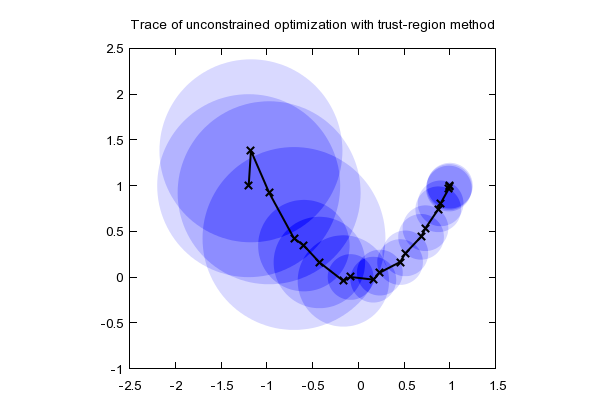
\includegraphics[width=0.6\textwidth]{img/TRM.png}
\end{figure}
\section{信赖域算法框架}
\begin{figure}[h!]
\caption{步长和改进方向都是预定信赖域大小的结果}
\centering
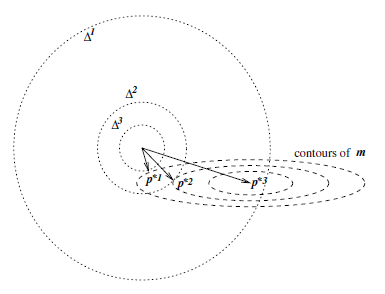
\includegraphics[width=0.6\textwidth]{img/TRM_stepsize.png}
\end{figure}
由带Lagrange余项的Taylor公式,有
\begin{equation*}
	f(x^k+d) = f(x^k) + \nabla f(x^k)^T d +\frac{1}{2}d^T\nabla^2 f(x^k+td)d,
\end{equation*}
其中$t\in (0, 1)$.我们用$f$的二阶近似来刻画$f(x)$在$x=x^k$的性质:
\begin{equation}\label{model_function}
	m_k(d) = f(x^k) +\nabla f(x^k)^Td + \frac{1}{2}d^TB^kd,
\end{equation}
$B^k$是对称矩阵,要求$B^k$是Hessian矩阵的近似.若$B^k$恰好是Hessian矩阵, 则$m_k(d)$的近似误差为$\mathcal{O}(||d||^3)$.\par
考虑到Taylor展开是函数的局部性质,于是我们仅在下面的求内考虑问题
\begin{equation*}
	\Omega_k = \{x^k + d\mid ||d||\leq \Delta_k\}
\end{equation*}
其中$\Delta_k$是一个与迭代有关的参数.我们称$\Omega_k$为\textbf{信赖域},$\Delta_k$为\textbf{信赖域步长}.我们相信在信赖域中$m_k(d)$能够很好地近似$f(x)$,因此信赖域算法每一步都要解决如下的子问题:
\begin{equation}\label{subp}
	\min\limits_{d\in \mathbb{R}^n} m_k(d),\quad s.t.\quad ||d||\leq \Delta_k.
\end{equation}
事实上,在信赖域算法中,选取信赖域半径至关重要,它决定了算法的收敛性.考虑到信赖域半径是“对模型函数$m_k(d)$相信的程度”,那么如果$m_k(d)$对函数$f(x)$近似较好,我们应扩大信赖域半径,反之就应该减小信赖域重新计算.我们引入如下的定义来衡量模型函数$m_k(d)$近似的好坏:
\begin{equation}\label{rho}
	\rho_k = \frac{f(x^k)-f(x^k+d)}{m_k(0)-m_k(d^k)},
\end{equation}
其中$d^k$为求解信赖域问题子问题\eqref{subp}得到的迭代方向.根据$\rho_k$的定义我们知道它即为函数值实际下降量与预估下降量的比值.如果$\rho_k$接近$1$,说明$m_k(d)$近似$f(x)$是比较成功的,我们应该扩大$\Delta_k$,否则应该缩小信赖域.
下面我们给出具体的算法,注意我们其实回避了如何求解子问题\eqref{subp}
\begin{algorithm}[H]
%\footnotesize%字体大小
\caption{信赖域算法}%首行显示算法名称
\begin{algorithmic}[1]%行编号,从Input, Output后面开始
%输入Input
\Require 最大半径$\Delta_max$,初始半径$\Delta_0$,初始点$x^0$,$k\leftarrow 0$.
\Require 给定参数$0\leq \eta < \bar{\rho_1}<\bar{\rho_2}<1$,$\gamma_1<1<\gamma_2$.

\While{未达到收敛准则}
\State 计算信赖域问题子问题\eqref{subp}得到迭代方向$d^k$(实际上是步长+方向).
\State 根据\eqref{rho}计算下降率$\rho_k$.
\If {$\rho < \bar\rho_1$}
	\State 缩小信赖域半径: $\Delta_{k+1}\leftarrow \gamma_1 \Delta_k$.
\Else
	\If{$\rho_k>\bar\rho_2$以及$||d^k||=\Delta_k$}
		\State 扩大信赖域半径:$\Delta_{k+1} \leftarrow \min\{\gamma_2\Delta_k, \Delta_{max}\}$.
	\Else
		\State 信赖域半径不变:$\Delta_{k+1}\leftarrow \Delta_k$	
	\EndIf
\EndIf
\If{$\rho_k> \eta$}
	\State 更新$x^{k+1} \leftarrow x^k+d^k$.
\Else
	\State $x^{k+1}\leftarrow x^k$.
\EndIf
\State $k\leftarrow k+1.$
\EndWhile
\end{algorithmic}  
\end{algorithm}
实际上,信赖域算法的大致思想就是首先判断模型函数$m_k(d)$是否是原函数$f(x)$在$\Delta_k$中的良好近似,并根据此修改信赖域半径.接着迈出步子走就好了.\par
我们通常取参数如下:$\bar\rho_1 = 0.25, \bar\rho_2=0.75$以及$\gamma_1=0.25, \gamma_2 = 2$.\par
下面我们给出求解信赖域子问题\eqref{subp}的算法.而这才是信赖域算法的关键.
\section{信赖域算法子问题求解}
信赖域子问题\eqref{subp}仅仅是一个涉及二次函数的约束优化问题,我们可以通过KKT条件求解,通过KKT条件得到最优解$d^*$应满足如下条件(过程太长, 详情参见文再文老师的书):
\begin{theorem}
	$d^*$是信赖域子问题
	\begin{equation*}
		\min\quad m(d) = f + g^Td+\frac{1}{2}d^TBd, \quad s.t.\quad ||d||\leq \Delta
	\end{equation*}
	的全局极小解当且仅当$d^*$可行且存在$\lambda\geq 0$满足
	\begin{equation}
		\begin{split}
			(B+\lambda I)d^* &= -g,\\
			\lambda(\Delta- ||d^*||) &= 0,\\
			(B+\lambda I)& \succeq 0.
		\end{split}
	\end{equation}
\end{theorem}
寻找子问题\eqref{subp}的近似解常有三种方法
\begin{enumerate}
	\item Cauchy点
	\item Dogleg算法(针对$B_k\succ 0$)
	\item 二维子空间极小化(对于$B_k$非正定)
\end{enumerate}
首先我们介绍Cauchy点
\subsection{Cauchy点}
\begin{definition}[Cauchy点]
	设$m_k(d)$是$f(x)$在点$x=x^k$处的二阶近似,常数$\tau_k$为如下优化问题的解
	\begin{equation*}
		\begin{split}
			&\min\quad m_k(-\tau \nabla f(x^k)),\\
			&s.t.\quad ||\tau \nabla f(x^k)||\leq \Delta_k, \tau\geq 0
		\end{split}
	\end{equation*}
	称$x_C^k\vcentcolon = x^k + d_C^k$为Cauchy点,其中$d_C^k = -\tau_k\nabla f(x^k)$.
\end{definition}
实际上,根据Cauchy点的定义, 它实际上是对$m_k(d)$进行一次精确线搜索的梯度法,只不过这个线搜索是考虑了信赖域约束的,参见下图
\begin{figure}[h!]
\caption{Cauchy点}
\centering
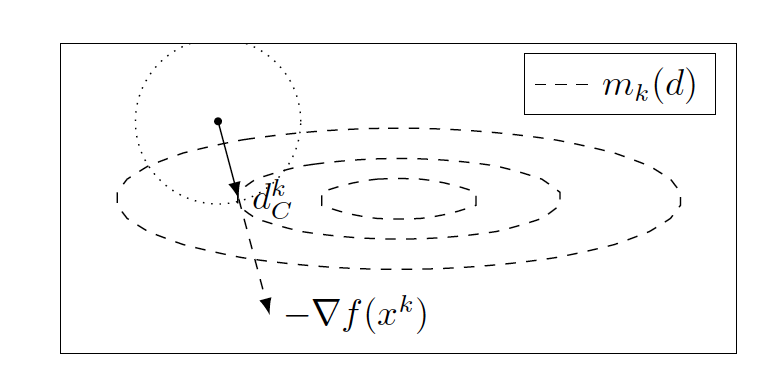
\includegraphics[width=0.6\textwidth]{img/cauchypoint.png}
\end{figure}
事实上, 根据定义,Cauchy点能够显式地计算出来,为方便起见,我们用$g^k$表示$\nabla f(x^k)$
\begin{equation*}
	\tau_k = \begin{cases}
		\frac{\Delta_k}{||g_k||}, & (g^k)^TB^kg^k\leq 0,\\
		\min\{\frac{||g^k||^2}{(g^k)^TB^kg^k},\frac{\Delta_k}{||g^k||}\}, &\text{其它}.
	\end{cases}
\end{equation*}
\subsection{dog leg 法}
Dog let法由Powell提出,结合了Gauss–Newton算法和梯度下降法,但是使用了显式信任区域。在每次迭代中,如果高斯-牛顿算法中的步骤位于信任区内,则将其用于更新当前解决方案。如果不是,则算法沿最陡的下降方向(称为柯西点)搜索目标函数的最小值。如果柯西点在信任区域之外,则将其截断到信任区域的边界,并将其作为新的解决方案。如果柯西点在信任区域内,则在信任区域边界与连接柯西点和Gauss-Newton步(dog leg step)的线之间的交点处采用新解。\par
\begin{note}
	我真的找不到太多dog leg法的资料, 它的slide味同嚼蜡看不懂.以后有心情再了解.
\end{note}